\documentclass[default]{beamer}
\setbeamertemplate{navigation symbols}{}
\setbeamertemplate{bibliography item}[text]

\usetheme{CambridgeUS}
\useoutertheme{infolines}
%\usecolortheme{crane}

\usepackage[utf8]{inputenc}					% Выбор языка и кодировки
\usepackage{csquotes}
\usepackage{tikz}
\usepackage{animate}
\usepackage{fp}
\usetikzlibrary{calc}
\usepackage{setspace}

\usepackage[
	language=auto,
	autolang=other,
	backend=biber,
	style=authortitle,
	sorting=ynt
]{biblatex}
\addbibresource{fierces.bib}
				
\DeclareSourcemap{
	\maps[datatype=bibtex, overwrite]{
		\map{
			\step[fieldset=langid, fieldvalue=english]
			\step[fieldset=doi, null]
			\step[fieldset=issn, null]
			\step[fieldset=isbn, null]
			\step[fieldset=url, null]
			\step[fieldsource=language, fieldset=langid, origfieldval]
		}
	}
}

\DeclareBibliographyDriver{std}{%
	\usebibmacro{bibindex}%
	\usebibmacro{begentry}%
	\usebibmacro{author/editor+others/translator+others}%
	\setunit{\labelnamepunct}\newblock
	\usebibmacro{title}%
	\newunit\newblock
	\usebibmacro{date}%
	\newunit\newblock
	\usebibmacro{finentry}
}
\DeclareBibliographyAlias{article}{std}
\DeclareBibliographyAlias{book}{std}
\DeclareBibliographyAlias{inproceedings}{std}
\DeclareBibliographyAlias{incollection}{std}

\graphicspath{{../../images/}} 			% Пути к изображениям

\makeatletter
\setbeamertemplate{footline}
{
	\leavevmode%
	\hbox{%
		\begin{beamercolorbox}[wd=.333333\paperwidth,ht=2.25ex,dp=1ex,center]{author
				in head/foot}%
			\usebeamerfont{author in
				head/foot}\insertshortauthor~~\beamer@ifempty{\insertshortinstitute}{}{(\insertshortinstitute)}
		\end{beamercolorbox}%
		\begin{beamercolorbox}[wd=.333333\paperwidth,ht=2.25ex,dp=1ex,center]{title in
				head/foot}%
			\usebeamerfont{title in head/foot}\insertshorttitle
		\end{beamercolorbox}%
		\begin{beamercolorbox}[wd=.333333\paperwidth,ht=2.25ex,dp=1ex,right]{date in
				head/foot}%
			\usebeamerfont{date in head/foot}Fierces on BICA --- \insertshortdate{}\hspace*{1em}
			\insertframenumber{}\hspace*{2ex} 
		\end{beamercolorbox}
	}%
	\vskip0pt%
}


\renewcommand*{\bibfont}{\tiny}

\begin{document}
	
	\title[Bio- and psycho-inspired modelling]{Biologically and psychologically inspired modelling in BICA}
	\author[Panov]{Aleksandr I. Panov}
	\institute[FRC CSC RAS]{Laboratory of Dynamic Intelligent Systems\\
		Federal Research Center ``Computer Science and Control''\\
		Russian Academy of Sciences}
	\date{22 April 2016} 
	
	\begin{frame}
		\titlepage
	\end{frame}

	\begin{frame}
		\frametitle{Self-presentation}
		\scriptsize
		\begin{columns}
			\begin{column}{0.85\textwidth}
				Aleksandr I. Panov, PhD
				\begin{itemize}
					\item Research Fellow in Laboratory of Dynamic intelligent systems of Federal Research Center ``Computer Science and Control'' of the	Russian Academy of Sciences.
					\item Research Fellow and Senior Lecturer in National Research University High School of Economics (Faculty of Computer Science)
					\item Assistant Lecturer in Moscow Institute of Physics and Technology (Department of Computer Science).
					\item Member of the Editorial Board of the Biologically Inspired Cognitive
					Architectures (BICA Journal).
					\item Regular Fellow of the Russian Association of the Artificial Intelligence (RAAI).
					\item Member of The Biologically Inspired Cognitive Architectures Society (BICA Society).
					\item Member of the NEURONET workgroup of the National Technology Initiative (ASI).
					\item Head of research projects for young scientists of Russian Foundation for Basic Research (RFBR).
				\end{itemize}
			\end{column}
			
			\begin{column}{0.15\textwidth}
				\centering
				\includegraphics[width=\textwidth]{advert/ras_en.png}
				\vspace{7pt}
				\includegraphics[width=0.7\textwidth]{advert/isa.png}
				\vspace{7pt}
				\includegraphics[width=0.5\textwidth]{advert/raai.png}
				\vspace{7pt}
				\includegraphics[width=0.5\textwidth]{advert/hse.png}
				\vspace{7pt}
				\includegraphics[width=\textwidth]{advert/mipt_en.jpg}
				\vspace{7pt}
				\includegraphics[width=\textwidth]{advert/bica2016.png}
				\vspace{7pt}
				\includegraphics[width=0.7\textwidth]{advert/asi_en.png}
			\end{column}
		\end{columns}
	\end{frame}

	\begin{frame}
		\frametitle{Research institute}
		
		\begin{columns}
			\begin{column}{0.6\textwidth}
				Federal Research Centre ``Computer Science and Control'' of \textbf{Russian Academy of Sciences}
				\par\bigskip
				\textbf{Includes}: Institute for Systems Analysis, Computational Center of Russian Academy of Sciences, Institute of Informatics Problems.
				\par\bigskip
				\textbf{R\&D areas}: Computer Science, Artificial Intelligence, Cognitive Psychology, Linguistics, Search Engines, Natural Language Processing, Cognitive Modelling, Control Systems, Computational Math, Patter Recognition, Data Analysis, Semiotics, Robotics, Economics.
			\end{column}
			\begin{column}{0.4\textwidth}
				\centering
				\includegraphics[width=0.7\textwidth]{misc/origin_ras.jpg}
				\vspace{10pt}
				\includegraphics[width=0.7\textwidth]{advert/isa_build.jpg}
			\end{column}
		\end{columns}
		
	\end{frame}
					
	\begin{frame}
		\frametitle{Nowadays BICA --- what is missing?}
		\begin{columns}
			\begin{column}{0.6\textwidth}
				\begin{itemize}
					\item Architectures for real robot control.
					\item Symbolic-subsymbolic processing.
					\item Integrated model of symbolic processing.
					\item Full multiagent integration.			
					\item Coalition management and formation.
					\item Human-robot interaction support.
				\end{itemize}
				\nocite{*}
				\printbibliography[keyword={please}, resetnumbers=true]
				
			\end{column}
			\begin{column}{0.4\textwidth}
				\begin{tikzpicture}
					\node[inner sep=0pt] at (1,0) {\includegraphics[width=0.7\textwidth]{misc/shakey}};
					\node[inner sep=0pt] at (-1,-3) {\includegraphics[width=0.7\textwidth]{misc/nao_hri}};										\node[inner sep=0pt] at (-1.3,2.3) {\includegraphics[width=0.6\textwidth]{misc/multi_agent}};						
					\node[inner sep=0pt] at (-1.2,0) {\tiny Shakey (Circa 1967)};
				\end{tikzpicture}
			\end{column}
		\end{columns}
	\end{frame}

	\begin{frame}
		\frametitle{STRL architecture}
		
		\begin{columns}
			\begin{column}{0.6\textwidth}
				\centering
				\includegraphics[width=\textwidth]{strl/strl_rita_eng}
			\end{column}
			\begin{column}{0.4\textwidth}
				3 levels of control:
				\begin{itemize}
					\item \textbf{Strategic}: Behavior planning (including inter-agent communication
					\item \textbf{Tactic}: Path planning (including prediction and monitoring)
					\item \textbf{Reactive}: Path following taking into account agent’s dynamic
				\end{itemize}
				\nocite{*}
				\printbibliography[keyword={strl}, resetnumbers=true]
			\end{column}
		\end{columns}
	\end{frame}

	\begin{frame}
		\frametitle{Reactive level: SDRE technique}
		\small
		\begin{itemize}
			\item Desired trajectory and UAV speed are received from the tactical level.
			\item Nonlinear control based on a special method of solving the State-Dependent Riccati Equation (SDRE).
			
		\end{itemize}
		\par\bigskip
		\centering
		\includegraphics[width=0.6\textwidth]{misc/plan_2}
		\nocite{*}
		\printbibliography[keyword={sdre}, resetnumbers=true]
	\end{frame}

	\begin{frame}
		\frametitle{Tactic level: 2 phases of path planning}
		\begin{columns}
			\begin{column}{0.7\textwidth}	
				\begin{enumerate}
					\item Path prediction (fast, no angle constraints)
					\begin{itemize}
						\item Using Theta* to find a path
						\item Use this path to calculate angle constraints (on reactive level)
					\end{itemize}
					\item Angle constrained path planning
					\begin{itemize}
						\item Using LIAN to find a path
						\begin{itemize}
							\item Not that fast
							\item No path can exist under constraint given
						\end{itemize}
					\end{itemize}
				\end{enumerate}
			\end{column}
			\begin{column}{0.3\textwidth}
				\centering
				\vspace{10pt}
				\includegraphics[width=\textwidth]{misc/plan_lian}
				\vspace{10pt}
				\includegraphics[width=0.5\textwidth]{strl/angl_constr_planning}
			\end{column}
		\end{columns}			
		\par\bigskip

		\nocite{*}
		\printbibliography[keyword={pathplan}, resetnumbers=true]

	\end{frame}
	
	\begin{frame}
		\frametitle{Strategic level: Sign knowledge representation}
		\small
		Sign as a component of knowledge:
		\begin{itemize}
			\item cultural-historical approach of Vygotsky-Luria
			\item the theory of activity of Leontiev
		\end{itemize}
		
		\begin{columns}
			\begin{column}{0.4\textwidth}
				\centering
				\includegraphics[width=\textwidth]{signs/sign_colored_rita.pdf}
			\end{column}
			\begin{column}{0.6\textwidth}
				\centering
				\includegraphics[width=0.7\textwidth]{signs/sign_kr.png}
			\end{column}
		\end{columns}
		
		This structure is supported by neuropsychological data (Edelmen, Ivanitsky, Mountcastle etc.)
		\nocite{*}
		\printbibliography[keyword={nerosign}, resetnumbers=true]
		
	\end{frame}

	\begin{frame}
		\frametitle{Sign world model}
		\centering
		\includegraphics[width=0.7\textwidth]{signs/sign_levels_en}
		
		\nocite{*}
		\printbibliography[keyword={swm}, resetnumbers=true]
	\end{frame}				
		
	\begin{frame}
		\frametitle{Sign world model}
		
		\begin{columns}
			\begin{column}{0.55\textwidth}
				\includegraphics[width=\textwidth]{signs/signs_net}
			\end{column}
			\begin{column}{0.45\textwidth}
				\textit{Semiotic network} $H=\langle H_P, H_A, H_M\rangle$ consisting of three semantic network: 
				\begin{itemize}
					\item $H_P=\langle2^P,\mathfrak R_P\rangle$ -- semantic network on the set of sign images,
					\item $H_P=\langle2^A,\mathfrak R_A\rangle$ -- semantic network on the set of sign meanings,
					\item $H_P=\langle2^M,\mathfrak R_M\rangle$ -- semantic network on the set of sign significances.
				\end{itemize}
				\nocite{*}
				\printbibliography[keyword={osipov}, resetnumbers=true]
			\end{column}
		\end{columns}
	\end{frame}				

	\begin{frame}
		\frametitle{Linking Operators}
		\centering
		\includegraphics[page=1,width=0.6\textwidth]{signs/oper_relat}
		
		Linking an image and a significance.
	\end{frame}		

	\begin{frame}
		\frametitle{Linking Operators}
		\begin{columns}
			\begin{column}{0.5\textwidth}
				\centering
				\includegraphics[page=2,width=\textwidth]{signs/oper_relat}
				
				Linking a significance and a meaning.
			\end{column}
			\begin{column}{0.5\textwidth}
				\centering
				\includegraphics[page=3,width=\textwidth]{signs/oper_relat}
				
				Linking a meaning and an image.
			\end{column}
		\end{columns}
	\end{frame}	
	
	\begin{frame}
		\frametitle{Sign Naming}
		\centering
		\includegraphics[width=0.5\textwidth]{signs/sign_naming_colored_en}
	\end{frame}		

	\begin{frame}
		\frametitle{Relations on sign components}
		\centering
		\includegraphics[page=1,width=0.8\textwidth]{signs/sign_relations}
		
		Similarity of images.
	\end{frame}	

	\begin{frame}
		\frametitle{Relations on sign components}
		
		\begin{columns}
			\begin{column}{0.3\textwidth}
				\centering
				Inclusion of images: 
				\par\bigskip
				\par\bigskip
				\par\bigskip
				\par\bigskip
				\par\bigskip
				Opposition of images: 
				
			\end{column}
			\begin{column}{0.7\textwidth}
				\includegraphics[page=2,width=0.8\textwidth]{signs/sign_relations}
				
				\includegraphics[page=3,width=0.8\textwidth]{signs/sign_relations}
			\end{column}
		\end{columns}
		
	\end{frame}	

	\begin{frame}
		\frametitle{Relations on sign components}
		\centering
		\includegraphics[page=4,width=0.7\textwidth]{signs/sign_relations}
		
		Script on significances.
	\end{frame}	

	\begin{frame}
		\frametitle{Relations on sign components}
		
		\begin{columns}
			\begin{column}{0.3\textwidth}
				\centering
				Subsumption of meanings: 
				\par\bigskip
				\par\bigskip
				\par\bigskip
				\par\bigskip
				\par\bigskip
				Opposition of meanings: 
				
			\end{column}
			\begin{column}{0.7\textwidth}
				\includegraphics[page=5,width=0.8\textwidth]{signs/sign_relations}
				\par\bigskip
				\includegraphics[page=6,width=0.8\textwidth]{signs/sign_relations}
			\end{column}
		\end{columns}
		
	\end{frame}	

	\begin{frame}
		\frametitle{Operations on sign components}
		
		\begin{columns}
			\begin{column}{0.5\textwidth}
				\centering
				\includegraphics[page=7,width=\textwidth]{signs/sign_relations}
				\par\bigskip
				Operation of closure on significances.
			\end{column}
			\begin{column}{0.5\textwidth}
				\includegraphics[page=8,width=\textwidth]{signs/sign_relations}
				\par\bigskip
				Operation of agglutination on meanings.
			\end{column}
		\end{columns}
	\end{frame}	

	\begin{frame}
		\frametitle{Model of goal-setting function}
		\centering
		\includegraphics[width=0.7\textwidth]{algo/goal_set_alg}
	\end{frame}	
											
	\begin{frame}
		\frametitle{Model of behavior planning function}
		\centering
		\includegraphics[width=\textwidth]{algo/plan_alg}
	\end{frame}	

	\begin{frame}
		\frametitle{Neural substrate}
		
		\begin{columns}
			\begin{column}{0.35\textwidth}
				\includegraphics[width=0.8\textwidth]{phisio/mozg_2}
				\par\bigskip
				\hspace{-7mm}\includegraphics[width=\textwidth]{phisio/mozg}
			\end{column}
			\begin{column}{0.65\textwidth}
				\includegraphics[width=\textwidth]{phisio/cortex_layers}
			\end{column}
		\end{columns}
		\nocite{*}
		\printbibliography[keyword={column}, resetnumbers=true]
	\end{frame}
	
	\begin{frame}
		\frametitle{Sign grounding assumptions}
		
		\begin{columns}
			\begin{column}{0.3\textwidth}
				\begin{figure}
					\includegraphics[width=\textwidth]{mpf/info_flow.jpg}
				\end{figure}
			\end{column}
			\begin{column}{0.7\textwidth}
				\begin{overlayarea}{\textwidth}{0.7\textheight}
					\only<1>{
						Hypothesis:
						\begin{itemize}
							\item neocortex consists of set of regions including set of columns, all regions are similar,
							\item columns are connected with lateral links,
							\item thalamus configures pattern sequences with inhibition and excitation processes.
						\end{itemize}
					}
					
					\only<2>{
						General features:
						\begin{itemize}
							\item all pattern sequences memorized in invariant form,
							\item all patterns are actualized associatively,
							\item all patterns are memorized in hierarchical form,
							\item feedback is used to predict input signal from low level.
						\end{itemize}
					}
					
					\only<3>{
						Simplifications:
						\begin{itemize}
							\item tim is discretized,
							\item simple hierarchy with links between neighborhoods only,
							\item all events have the same duration in time,
							\item we use threshold model of decision process in the case of uncertainty,
							\item all unexpected signals are inhibited,
							\item we don't use motor part of feedback loop (meaning component).
						\end{itemize}
					}				
				\end{overlayarea}
			\end{column}
		\end{columns}
	\end{frame}
	
	\begin{frame}
		\frametitle{Formal neuron model}
		
		\begin{center}
			\includegraphics[width=0.9\textwidth]{phisio/neuro_htm}
		\end{center}
		
		\begin{itemize}
			\item A segment of proximal dendrite "--- direct activation.
			\item Segments of distal dendrite "--- lateral input and prediction state.
		\end{itemize}
	\end{frame}
	
	\begin{frame}
		\frametitle{Hierarchy of neuron ensembles}
		
		\begin{columns}
			\begin{column}{0.5\textwidth}
				\includegraphics[width=0.9\textwidth]{mpf/hierarchy}
			\end{column}
			\begin{column}{0.5\textwidth}
				\includegraphics[width=0.9\textwidth]{mpf/hierarchy_conv}
			\end{column}
		\end{columns}
		
	\end{frame}
	
	\begin{frame}
		\frametitle{Hierarchical model}
		
		
		\begin{overlayarea}{\textwidth}{\textheight}
			\only<1>{
				\begin{center}
					\includegraphics[width=0.7\textwidth]{mpf/hawkins_htm}
				\end{center}
			}
			\only<2>{
				\centering
				\includegraphics[width=0.8\textwidth]{mpf/hawkins_htm_ex}
			}
		\end{overlayarea}
	\end{frame}
	
	\begin{frame}
		\frametitle{Layered organization}
		
		\begin{columns}
			\begin{column}{0.65\textwidth}
				\includegraphics[width=0.9\textwidth]{mpf/regions_connect}
			\end{column}
			\begin{column}{0.35\textwidth}
				\includegraphics[width=\textwidth]{phisio/column}
			\end{column}
		\end{columns}
	\end{frame}
	
	\begin{frame}
		\frametitle{Sign components}
		
		When learning process finished set of synapses defines both vertical connections between nodes and horizontal connections within a node.
		\par\bigskip
		Each node is modeled with set of prediction matrices formed in a result of learning process within memory prediction framework.
	\end{frame}
			
	\begin{frame}
		\frametitle{Algorithm $\mathfrak A_{th}$ of sign component actualization}
		
		\begin{tikzpicture}[overlay,remember picture]
		
		\tikzstyle{z_matrix} = [draw, rectangle, minimum width = 60, minimum height = 60,fill=white];
		
		\onslide<1->{
			\node (meas_fun) at (0.7,0.5) {$\hat f_1,\hat f_2\dots,\hat f_k$};	
		}
		\onslide<2->{
			\node (control_vect) at ($(meas_fun)+(-0.5,1.2)$) {$\hat x^{j+1}$};
			\path[->,thick,red] (control_vect.east)  edge[out = -45, in = 45, right] (meas_fun.north); 
		}
		\onslide<3->{
			\node[z_matrix] (z_1) at ($(meas_fun)+(2.6,-0.5)$) {};
			\node[z_matrix] at ($(z_1)+(0.2,-0.1)$) {};
			\node[z_matrix] at ($(z_1)+(0.4,-0.2)$) {};
			
			\node[z_matrix] at ($(z_1)+(0.9,-0.5)$) {};
			\node[z_matrix] at ($(z_1)+(1.1,-0.6)$) {};
			\node[z_matrix] at ($(z_1)+(1.3,-0.7)$) {};
			
			\path[->,thick,blue] ([xshift=20]meas_fun.south)  edge[out = -90, in = -155, right] ($(z_1)+(-1,-1.2)$);
			\path[->,thick,blue] ([xshift=-25]meas_fun.south)  edge[out = -90, in = -155, right] ($(z_1)+(-0.1,-1.7)$);
			
			\node at ($(z_1)+(-1,1.4)$) {$Z^*$};
			
			\node at ($(z_1)+(0.8,1.4)$) {$Z_1$};
			\node at ($(z_1)+(1.4,1.2)$) {$\ddots$};
			\node at ($(z_1)+(2,0.9)$) {$Z_k$};
		}
		
		\onslide<4->{
			\draw[ultra thick, green!60!black] ($(z_1)+(-0.4,-1.1)$) -- ($(z_1)+(-0.4,0.6)$);
			\draw[ultra thick, green!60!black] ($(z_1)+(0.5,-1.6)$) -- node[right,black] {$z_1^r$} ($(z_1)+(0.5,0.1)$);
			
			\draw[->, thick, green!60!black] ($(z_1)+(-0.1,-3)$) -- node[right,black] {$\bar x(0)$} ($(z_1)+(-0.1,-2)$);
		}
		
		\onslide<5->{
			\node[z_matrix] (z_2) at ($(z_1)+(5,0)$) {};
			\node[z_matrix] at ($(z_2)+(0.2,-0.1)$) {};
			
			\node[z_matrix] at ($(z_2)+(0.9,-0.5)$) {};
			\node[z_matrix] at ($(z_2)+(1.3,-0.7)$) {};
			
			\node at ($(z_2)+(-1,1.4)$) {$Z^*$};
			\node at ($(z_2)+(0.8,1.4)$) {$Z_1$};
			\node at ($(z_2)+(1.4,1.2)$) {$\ddots$};
			\node at ($(z_2)+(2,0.9)$) {$Z_k$};
			
			\draw[->, ultra thick] ($(z_1)+(2.6,-0.6)$) -- node [above] {\scriptsize$\frac{\|\bar z_1^r-\bar x(0)\|}{\|\bar z_1^r\|+\|\bar x(0)\|}$} ($(z_1)+(3.7,-0.6)$);
			
			\draw[ultra thick, dotted, green!60!black] ($(z_2)+(-0.6,-1)$) -- ($(z_2)+(-0.6,0.7)$);
			\draw[ultra thick, dotted, green!60!black] ($(z_2)+(0.5,-1.6)$) -- ($(z_2)+(0.5,0.1)$);
		}
		
		
		\onslide<6->{
			\draw[->, thick, red] ($(z_2)+(0.3,1.4)$) -- node[right,black] {$\bar x^*(0)$} ($(z_2)+(0.3,3)$);
		}
		
		\onslide<7>{
			\draw[<-, thick, red] ($(z_2)+(-0.1,-3)$) -- node[right,black] {$\hat x^j(0)$} ($(z_2)+(-0.1,-2)$);
		}
		
		\onslide<7->{				
			\draw[ultra thick, green!60!black] ($(z_2)+(-0.4,-1)$) -- ($(z_2)+(-0.4,0.7)$);
			\draw[ultra thick, green!60!black] ($(z_2)+(0.7,-1.6)$) -- node[right,black] {$z_2^r$} ($(z_2)+(0.7,0.1)$);	
		}
		\onslide<8->{
			\draw[->, thick, green!60!black] ($(z_2)+(-0.1,-3)$) -- node[right,black] {$\bar x(1)$} ($(z_2)+(-0.1,-2)$);
		}
		
		\onslide<9->{
			\draw[->, ultra thick] ($(z_2)+(2.6,-0.6)$) -- node [above] {\scriptsize$\frac{\|\bar z_1^r-\bar x(1)\|}{\|\bar z_1^r\|+\|\bar x(1)\|}$} ($(z_2)+(3.7,-0.6)$);
		}
		\end{tikzpicture}
	\end{frame}
	
	\begin{frame}
		\frametitle{Behavior planning algorithm}
		
		\begin{columns}
			\begin{column}{0.7\textwidth}
				\includegraphics[width=\textwidth]{strl/beh_plan-0.png}
			\end{column}
			\begin{column}{0.3\textwidth}
				\tiny
				Planning starts from final situation and aims to meet start situation.
				\par\bigskip
				Main steps of algorithm (MAP iteration):
				\begin{itemize}
					\item \textit{M-step} -- search of relevant significances,
					\item \textit{A-step} -- choose a personal meaning from the set of personal meanings corresponding to the found significances,
					\item \textit{P-step} -- construct the new current situation using the set of features from the condition of performed action,
					\item \textit{S-step} -- send a message to other members of the coalition  or perform the action corresponding to the chosen personal meaning or execute action hierarchy up to \color{red} path planning operations.
				\end{itemize}
			\end{column}
		\end{columns}
		\nocite{*}
		\printbibliography[keyword={behplan}, resetnumbers=true]
	\end{frame}	
	
	\begin{frame}
		\frametitle{Smart Relocation Tasks (SRT)}
		
		\begin{columns}
			\begin{column}{0.55\textwidth}
				\begin{center}
					\includegraphics[page=1,width=0.85\textwidth]{examples/slides_colored}
				\end{center}
				
				\textbf{Problem}
				
				Goal area can not be achieved by some agents on their own (using standalone task and path planning methods)
				
				\textbf{Solution}
				
				Agents must communicate and some agents must alter their ``selfish'' plans in order to construct coalition plan
				
			\end{column}
			\begin{column}{0.45\textwidth}
				3 levels of control:
				\begin{itemize}
					\item Transformable environment
					\item Different types of obstacles (some -- can be destroyed)
					\item Agents with different capabilities (some agents can destroy obstacles, others -- can not)
					\item Common spatial goal (ALL agents must reach this region in order goal to be achieved)
				\end{itemize}
			\end{column}
		\end{columns}
	\end{frame}

	\begin{frame}
		\frametitle{Model task}
		
		\begin{figure}
			\includegraphics[width=\textwidth]{examples/rita_ex_proc.png}
		\end{figure}
	\end{frame}

	\begin{frame}
		\frametitle{Spatial knowledge representation}
		
		Relocation actions --- signs $s_t$ (features $f_t$, $t$ --- relocation type), with corresponding prediction matrices $Z_t$ consist of 3 columns:
		\[
		z_1=(l_x, I), z_2=(l_y, d_u, E), z_3=(l_y, I, t_v),
		\]
		\begin{itemize}
			\item $l_x$, $l_y$ --- features represented category of distance in a spatial logic (e.g., ``far'', ``closely'' etc.), 
			\item $d_u$ --- features represented category of direction in a spatial logic (e.g., ``left'', ``straight'' etc.), 
			\item $t_v$ --- features represented category of time in temporal logic (e.g., ``soon'', ``not soon'' etc.),
			\item $I$ --- feature of agent presence, 
			\item $E$ --- feature of obstacle absence.
		\end{itemize}
	\end{frame}
			
	\begin{frame}
		\frametitle{Model task}
		\begin{center}
			\scalebox{0.7}{
				\animategraphics{12}{examples/slides_colored}{}{}			
			}
		\end{center}
	\end{frame}

	\begin{frame}
		\frametitle{Interaction with Behavior planning}
		
		\begin{enumerate}
			\item Non-angle-constrained path can not be found
			\begin{itemize}
				\item It takes a while to come to that
				\item Identify blocking obstacle
				\item Pass id (or coordinates) of that obstacle to upper level of control
				\begin{itemize}
					\item On upper level: messaging for help, altering the coalition plan
				\end{itemize}
			\end{itemize}
			\item Non-angle-constrained path can is found but angle-constrained is not
			\begin{itemize}
				\item Agent can not reach goal area under current constraints (time, speed etc.)
				\item Inform upper level of control and ask for a task update (setting new time constraints for example)
			\end{itemize}
		\end{enumerate}
	\end{frame}
	
	\begin{frame}
		\frametitle{Case study}
		
		\begin{center}
			\includegraphics[page=1,width=0.85\textwidth]{examples/slides_colored}
		\end{center}
		\par\bigskip
		Activated signs for agent $A_1$: ``place $X_6$'', ``far'', ``move 1'' $\rightarrow$ \color{red} path planning operations.
	\end{frame}
	
	\begin{frame}
		\frametitle{Case study}
		
		\begin{center}
			\includegraphics[page=31,width=0.85\textwidth]{examples/slides_colored}
		\end{center}
		\par\bigskip
		Activated signs for agent $A_1$: ``obstacle 1'', ``near'', ``place $X_6$''.
	\end{frame}
	
	\begin{frame}
		\frametitle{Case study}
		
		\begin{center}
			\includegraphics[page=42,width=0.85\textwidth]{examples/slides_colored}
		\end{center}
		\par\bigskip
		Activated signs for agent $A_1$: ``send message'', ``agent $A_2$''.
	\end{frame}
	
	\begin{frame}
		\frametitle{Case study}
		
		\begin{center}
			\includegraphics[page=58,width=0.85\textwidth]{examples/slides_colored}
		\end{center}
		\par\bigskip
		Activated signs for agent $A_2$: ``place $Y_3$'', ``far'', ``move 2'' $\rightarrow$ \color{red} path planning operations.
	\end{frame}
	
	\begin{frame}
		\frametitle{Case study}
		
		\begin{center}
			\includegraphics[page=95,width=0.85\textwidth]{examples/slides_colored}
		\end{center}
		\par\bigskip
		Activated signs for agent $A_2$: ``place $Y_1$'', ``near'', ``obstacle 1'', ``destroy''.
	\end{frame}
	
	\begin{frame}
		\frametitle{Case study}
		
		\begin{center}
			\includegraphics[page=116,width=0.85\textwidth]{examples/slides_colored}
		\end{center}
		\par\bigskip
		Activated signs for agents $A_1$ and $A_2$: ``far'', ``move 3'' $\rightarrow$ \color{red} path planning operations.
	\end{frame}
	
	\begin{frame}
		\frametitle{Case study}
		
		\begin{center}
			\includegraphics[page=171,width=0.85\textwidth]{examples/slides_colored}
		\end{center}
		\par\bigskip
		Activated signs for agents $A_1$ and $A_2$: goal state (``place G'').
	\end{frame}
		
	\begin{frame}
		\centering
		\Huge
		Thank you for attention!
		\normalsize
		\par\bigskip
		\par\bigskip
		FRC CSC RAS
		\par\bigskip
		pan@isa.ru, panov@bicasociety.org
		\par\bigskip
		\url{https://www.hse.ru/en/staff/apanov}
	\end{frame}
														
%	\begin{frame}
%		\frametitle{Цели курса}
%		
%		\begin{columns}
%			\begin{column}{0.5\textwidth}
%				
%			\end{column}
%			\begin{column}{0.5\textwidth}
%				\begin{figure}
%					\includegraphics[width=\textwidth]{logo}
%				\end{figure}
%			\end{column}
%		\end{columns}
%	\end{frame}
	%	\begin{frame}
	%		\frametitle{Цели курса}
	%		
	%		\begin{itemize}
	%			\item
	%		\end{itemize}
	%	\end{frame}
	
\end{document}
	
	
